\chapter{Tätigkeitsbereiche und Aufgaben}
\label{sec:main}
\section{Überblick}
\label{sec:main:overview}
Ich habe im Rahmen meines Praktikums am Projekt \textit{SD4M - Smart Data for Mobility} mitgearbeitet.
Meine konkrete Aufgabe war die Aufbereitung und Integration verschiedener Daten und Datenbanken, damit diese im Projekt Verwendung finden konnten. Meine Hauptdatenquelle waren die Geodaten des OpenStreetMap\footnote{http://www.openstreetmap.org/} Projekts.
\subsection{Das Projekt SD4M}
\label{sec:main:overview:sd4m}
Das Projekt \textit{Smart Data for Mobilty}\footnote{http://sd4m.net/}, im folgenden \textit{SD4M} genannt, ist ein Verbundprojekt eines Konsortiums aus 5 Partnern und wird vom Bundesministerium für Wirtschaft und Energie gefördert.
Das Konsortium besteht aus 4 Wirtschaftsunternehmen und dem DFKI als Forschungseinrichtung.
\begin{compactitem}
  \item DB Systel GmbH (Konsortialführung)
  \item Deutsches Forschungszentrum für Künstliche Intelligenz GmbH
  \item idalab GmbH
  \item ]init[ AG für digitale Kommunikation
  \item PS-Team Deutschland GmbH & Co. KG
\end{compactitem}
Ziel des SD4M Projekts ist eine branchenübergreifende Serviceplattform, welche Daten der unterschiedlichen Mobilitätsanbieter (z.B. den Fahrplan der Deutschen Bahn) sowie öffentlich verfügbare strukturierte und unstrukturierte Daten (z.B. Twitter oder Facebook) miteinander verknüpft.
Diese verknüpften Daten sind für Endnutzer, aber auch für Unternehmen oder die öffentliche Verwaltung von Interesse.
In Abbildung \ref{fig:tweetXfahrplan} wird verdeutlicht, wie sich aus unstrukturierten Twitter-Daten Verspätungsinformationen für konkrete Verkehrsmittel extrahieren lassen.
Diese können dann Endnutzern oder den Mobilitätsanbietern zur Verfügung gestellt werden.
\begin{figure}
   \centering
   \fbox{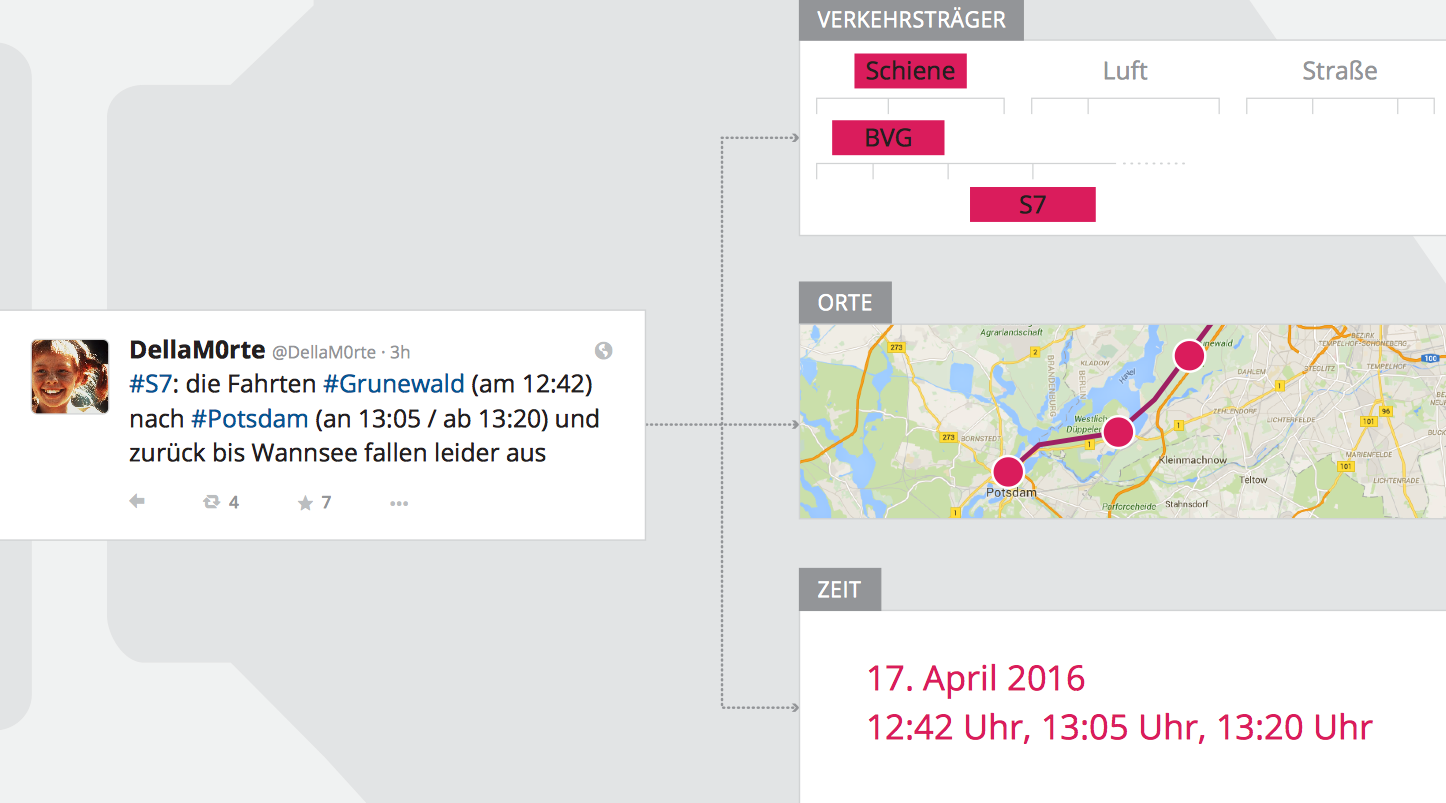
\includegraphics[width=1\textwidth]{gfx/sd4m_praesi_1.png}}
   \caption{Verknüpfung eines Tweets mit Fahrplandaten\protect\cite{WEB:SD4M:Presentation:2016}}
   \label{fig:tweetXfahrplan}
 \end{figure}

\section{Vorbereitung}
\label{sec:main:preparation}
Beim ersten Gespräch mit meinem Praktikumsbetreuer Dr. Philippe Thomas informierte ich mich, welche Programmierumgebungen und Programmiersprachen beim DFKI üblich sind.
Ebenfalls erkundigte ich mich nach einer vorhandenen OpenStreetMap Datenbank und weiterer vorhandener Infrastruktur.
Wir klärten, dass Java die geeignetste Sprache zur Lösung meiner Aufgaben war.
Ebenfalls war eine OpenStreetMap Datenbank mit dem Datenbestand von Deutschland, sowie ein GitLab Repository Server vorhanden.
Da ich auf meinem eigenen Notebook entwickeln wollte, installierte ich mir einen virtuellen Linux-Server mit einer PostgreSQL Datenbank um einen kleinen Teil der OpenStreetMap Daten lokal auf meinem Rechner zu haben.
So konnte ich schneller entwickeln und mit einer wesentlich kleineren Datenbank testen.
Als Java-Entwicklungsumgebung entschied ich mich für \textit{JetBrains IntelliJ IDEA}\footnote{https://www.jetbrains.com/idea/} und zur Arbeit mit den Datenbanken für \textit{JetBrains DataGrip 2016}\footnote{https://www.jetbrains.com/datagrip/}.

\section{Aufgaben}
Meine Aufgaben während des Praktikums lassen sich in drei Teilbereiche gliedern. Zunächst sollte ich eine Straßenliste aus OpenStreetMap extrahieren. Anschließend verknüpfte und aggregierte ich Daten, welche von der Deutschen Bahn geliefert wurden, mit Daten aus OpenStreetMap. In den letzten Wochen meiner Praxisphase gab es dann noch verschiedene Datenaufwertungs- und aufbereitungsaufgaben. Auf diese drei Themengebiete wird in diesem Abschnitt eingegangen.

\subsection{Extraktion einer Straßenliste aus OpenStreetMap}

\subsubsection{Aufgabe}
Meine erste Aufgabe bestand darin, eine Liste aller Straßen Deutschlands inklusive dazugehöriger Geodaten zu erstellen.
Es sollte eine Java Anwendung erstellt werden, welche via Kommandozeilenargumenten konfiguriert wird und die entsprechenden Ergebnisse in einer CSV-Datei ablegt.
Im Ergebnis sollten pro zusammenhängendem Straßensegment die Daten
\begin{compactitem}
  \item \textbf{ID}, eine fortlaufende Nummer
  \item \textbf{Name}, der Name der Straße
  \item \textbf{LineString}, der geographische Straßenverlauf im \textit{Well-Known-Binary (WKB)} Format (siehe Anlage \ref{sec:appendix:wkb})
  \item \textbf{GeoJSON}, der geographische Straßenverlauf im \textit{GeoJSON} Format (siehe Anlage \ref{sec:appendix:geojson})
\end{compactitem}
vorhanden sein.
Diese Daten sollten anschließend zur geographischen Verortung von Straßen aus Tweets genutzt werden.
Eine Beispielausgabe des fertigen Programms findet sich in Anhang~\ref{sec:appendix:ose:output}.

\subsubsection{Lösung}

Für meinen Anwendungsfall, die Filterung und Extraktion von Daten, war es notwendig, die OpenStreetMap Daten in einer Datenbank vorliegen zu haben.
Der Hauptgrund hierfür ist dem Datenformat der OpenStreetMap Daten geschuldet. Wie im Anhang \ref{sec:appendix:osm:data} aufgezeigt, beinhalten die OpenStreetMap Daten \textit{Nodes} (Punkte mit Koordinaten) und \textit{Ways} (Linien aus Punkten).
Importwerkzeuge, welche eine Datenbank aus OpenStreetMap Daten erstellen, haben die nützliche Eigenschaft, die Koordinaten aller Punkte eines Weges zu aggregieren.
Das ermöglicht die direkte Extraktion der Geometrie eines Ways ohne sich für jeden Way die Koordinaten aus den Daten selbst aggregieren zu müssen.
Die zwei populärsten Importwerkzeuge zur Erstellung einer Datenbank aus OpenStreetMap Daten sind hierbei \textbf{osm2pgsql}\footnote{https://github.com/openstreetmap/osm2pgsql}\label{osm2pgsql} und \textbf{Osmosis}\footnote{https://github.com/openstreetmap/osmosis}.
Beide erzeugen unterschiedliche Datenbankschemata.

Das DFKI besitzt Datenbanken, in denen die OpenStreetMap Daten Deutschlands mit osm2pgsql sowie Osmosis importiert wurden.
Ich informierte mich darüber, welches Schema am verlustfreisten ist.
\begin{quote}
``osm2pgsql is mainly written for rendering data with data. So it only imports tags which are going to be useful for rendering. ... whereas osmosis and osmium more geared towards truthfully representing a full OSM data set.'' \cite{WEB:Giswiki:Osm2pgsql:2015}
\end{quote}

Ich entschied mich für die Datenbank im Osmosis-Schema, da diese den wahren Datenbestand am besten repräsentiert.

Eine physikalisch vorhandene Straße wird durch mehrere aneinanderhängende \textit{Ways} repräsentiert.
Wenn sich im Straßenverlauf ein Attribut (Ein \textit{Tag}) der Straße ändert, zum Beispiel die zulässige Höchstgeschwindigkeit, muss ein neues Teilstück diese neuen Gegebenheiten abbilden.
Ein Beispiel dafür findet sich sich in Anlage \ref{sec:appenix:osm:streets}.
Das Ziel war nun, eine Liste zusammenhängender Ways mit gleichem Name zu aggregieren und diese zu exportieren. Dazu plante ich folgenden Ablauf:

\begin{compactenum}
  \item Ermittlung aller Straßennamen aus der Datenbank
  \item Abfrage aller Ways pro Straßenname
  \item Trennung zusammenhängender Ways in Gruppen
  \item Aggregation der geographischen Informationen aller Ways einer Gruppe
  \item Export in Zieldatei
\end{compactenum}

Als kompliziertestes Problem stellte sich die Trennung zusammenhängender Way-Gruppen dar.
In Abbildung~\ref{fig:ose:osm_streetgroups_1} ist ein Kartenausschnitt mit allen Ways mit dem Name \textit{``Berliner Straße''} dargestellt.
\begin{figure}[htb]
   \centering
   \fbox{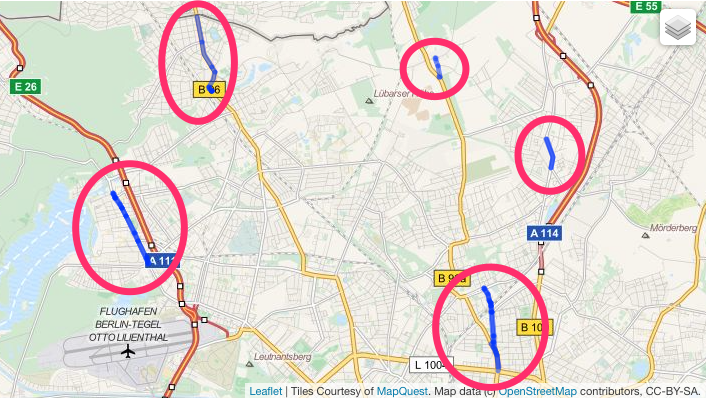
\includegraphics[width=1\textwidth]{gfx/osm_streetgroups_1.png}}
   \caption{Kartenauszug verschiedener Straßengruppen am Beispiel ``Berliner Straße''}
   \label{fig:ose:osm_streetgroups_1}
 \end{figure}
In diesem sind 5 Way-Gruppen erkennbar.
Optisch ist das Problem der Trennung einfach zu lösen, jedoch war mir nicht auf Anhieb klar wie ich das programatisch lösen sollte.
Ich habe die Problemstellung dann weiter abstrahiert und kam auf die Idee die Ways und die dazugehörigen Nodes als Graph zu verstehen. Schematisch ist das in Abbildung~\ref{fig:ose:osm_streetgroups_2} dargestellt.
\begin{figure}[htb]
   \centering
   \fbox{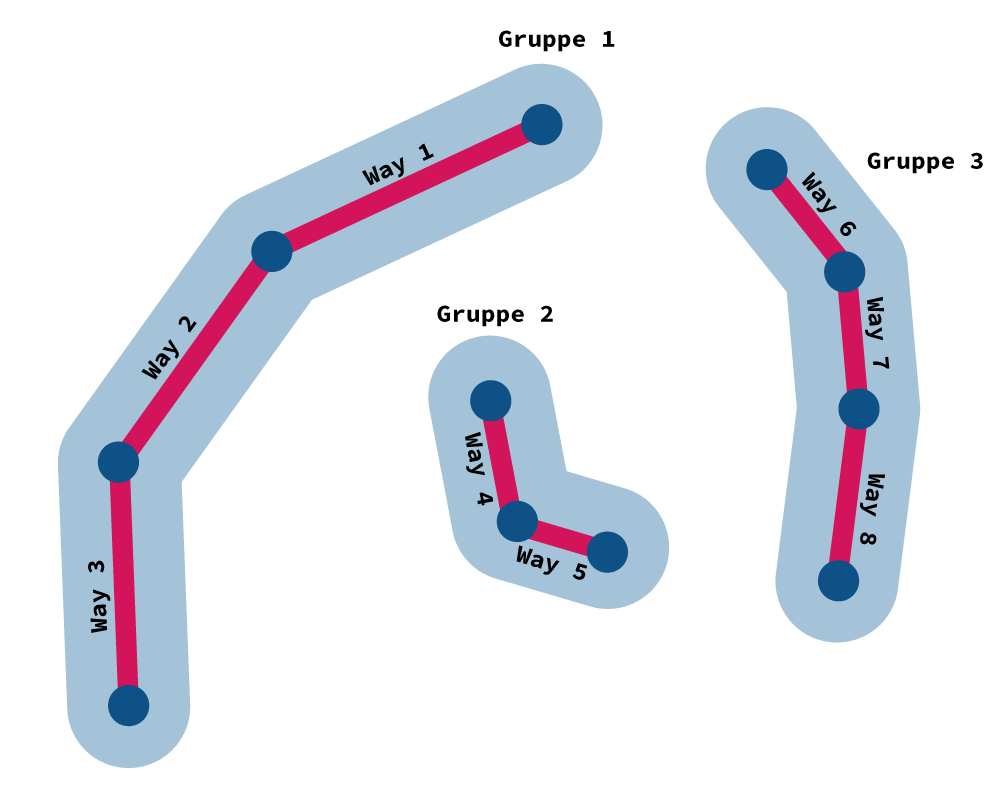
\includegraphics[width=0.8\textwidth]{gfx/osm_streetgroups_2.png}}
   \caption{Schematische Darstellung des Problems der Weggruppenfindung}
   \label{fig:ose:osm_streetgroups_2}
 \end{figure}
Ich ging davon aus, dass dieses Graphen-Problem von einer bestehenden Graphen-Bibliothek gelöst werden kann und fand \textit{JGraphT}\footnote{http://jgrapht.org}.
Mit JGraphT konnte ich alle Nodes als Knoten und alle Ways als Kanten in einem Graph abbilden.
Anschließend konnte der Graph auf zusammenhängende Elemente untersucht und getrennt werden.
Ein kurzes Beispiel zur Verwendung von JGraphT zur Trennung eines Graphen in separate verbundene Teile wird in Anhang \ref{sec:appendix:jgrapht_separation} gezeigt.
Schwierig war hierbei allerdings dass nur Mengen von zusammenhängenden Knoten zurückgegeben wurden, die Kanten jedoch verloren gingen.
Ich musste mir also im Voraus die Verbindungen der einzelnen Knoten speichern und diese anschließend erneut verarbeiten.
Der vollständige Quellcode der entsprechenden Klasse \texttt{GraphSeparator.java} ist in Anhang~\ref{sec:appenix:ose:graphseparator} angefügt.

\subsubsection{Programmstruktur}
Für viele Problemstellungen innerhalb des erstellten Programms wurden externe Bibliotheken verwendet (Siehe Tabelle \ref{tab:OsmosisStreetExtractor:Libraries}).
Die Ahängigkeiten wurden mit \textit{Apache Maven}\footnote{http://maven.apache.org} verwaltet.
\begin{table}[htb]
\centering
\caption{verwendete externe Bibliotheken}
\label{tab:OsmosisStreetExtractor:Libraries}
\begin{tabular}{|l|l|}
\hline
\textbf{Problem}                          & \textbf{verwendete Bibliothek}     \\ \hline
Datenbankanbindung PostgreSQL             & PostgreSQL JDBC Driver JDBC 4.1    \\ \hline
Verarbeitung von Kommandozeilenargumenten & Apache Commons CLI                 \\ \hline
Verarbeitung von JSON Objekten            & com.googlecode.json-simple         \\ \hline
Aufbau eines Graphen                      & org.jgrapht.jgrapht-core           \\ \hline
\end{tabular}
\end{table}

\begin{figure}[htb]
   \centering
   \fbox{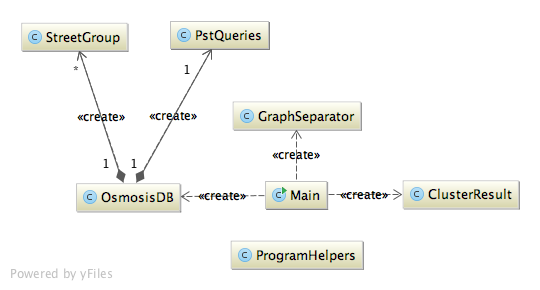
\includegraphics[width=1\textwidth]{gfx/ose_uml.png}}
   \caption{Klassendiagramm des fertigen Programms}
   \label{fig:ose:uml}
 \end{figure}

Das Programm erhielt den Namen \textbf{\texttt{OsmosisStreetExtractor}}. Die Struktur wird in Abbildung~\ref{fig:ose:uml} gezeigt.
Die Klasse \texttt{Main} erzeugt eine Instanz vom Typ \texttt{OsmosisDB} welche die Datenbankverbindung verwaltet.
Innerhalb von \texttt{OsmosisDB} werden nun alle Straßennamen Deutschlands ermittelt und in einer Liste aus \texttt{StreetGroup} Instanzen gespeichert.
Anschließend verarbeitet \texttt{Main} alle \texttt{StreetGroup} Objekte und sendet sie zur Trennung in zusammenhängende Segmente an den \texttt{GraphSeparator}.
Die nun getrennten Ergebnisse pro Straßenname werden in Instanzen vom Typ \texttt{ClusterResult} abgelegt, welche dann in die Ausgabedatei geschrieben werden.
Die Klasse \texttt{PstQueries} hält alle \texttt{PreparedStatements} für die Datenbankabfragen.

Eine Beispielausgabe des Programms findet sich in Anhang~\ref{sec:appendix:ose:output}.

\subsubsection{Schwierigkeiten}
Das Testen auf einer kleinen Datenbank beschleunigte zwar die Entwicklung, aber erst der erste Test auf der Hauptdatenbank zeigte massive Performanceprobleme auf.
Ich wollte meine Anwendung möglichst speicherschonend gestalten und fragte die Ways zu den separaten Straßennamen  einzeln aus der Datenbank ab.
Dies funktionierte auf meiner lokalen und wesentlich kleineren Testdatenbank sehr gut, jedoch auf der Datenbank mit den gesamten Daten Deutschlands annähernd gar nicht.
Eine Messung zeigte dass die Abfragen auf der Deutschland-Datenbank mit 300ms Abfragezeit der Flaschenhals waren.
Ich schrieb letztendlich die Datenbankanbindungsklasse \texttt{OsmosisDB} fast komplett um.
Statt vieler kleiner Abfragen, welche wenig Daten zurücklieferten, wurden nun wenige Abfragen an die Datenbank gestellt, die jedoch viele Daten lieferten.
Die Verarbeitung erfolgte dann komplett im Arbeitsspeicher und war performant genug.\\\\
Ebenfalls dauerte es eine Weile bis ich die Trennung der einzelnen Straßengruppen als Graphenproblem verstand.

\subsection{Verknüpfung von Daten der Deutschen Bahn mit Daten aus OpenStreetMap}
\subsubsection{Aufgabe}
Das DFKI arbeitet mit Daten, welche von der Deutschen Bahn bereitgestellt wurden, die alle größeren Bahnhöfe Deutschlands, sowie die Linien und Abfahrtszeiten aller Zugverbindungen enthalten.
Diese liegen im \textit{General Transit Feed Specification (GTFS)} Format\footnote{https://developers.google.com/transit/gtfs/} vor, einem Datenformat zur Veröffentlichung von Fahrplänen und dazugehörigen Informationen wie zum Beispiel geographischer Positionen der Bahnhöfe. Hierzu ist auch eine kurze Beschreibung in Anhang \ref{sec:appendix:gtfs_spec} verfügbar.

Meine Hauptaufgabe bestand darin, eine Abbildung von Bahnhöfen aus den GTFS-Daten der Deutschen Bahn (im folgenden DB-GTFS Daten genannt) auf Objekte aus den OpenStreetMap Daten zu erstellen.
Mit Hilfe dieser Abbildung ist es möglich, zu Bahnhöfen oder Zugstrecken erweiterte Informationen aus OpenStreetMap zu beziehen, wie zum Beispiel das Bundesland oder Straßen in der Nähe des Bahnhofes.

Als Nebenaufgabe sollte geprüft werden, inwiefern sich aus den kombinierten Daten ein geographisch exakter Streckenverlauf eines Zuges für die graphische Darstellung ermitteln lässt.

\subsubsection{Lösung}
Da GTFS-Daten nur aus Textdateien bestehen, sollten diese zur effizienten Verarbeitung in einer Datenbank vorhanden sein.
Das DFKI hatte die DB-GTFS Daten bereits in einer Datenbank vorliegen, jedoch wollte ich eine lokale Kopie in meiner eigenen Entwicklungsumgebung.
Zum Import wurde der frei verfügbare Importer \textit{OpenTransitTools/gtfsdb}\footnote{https://github.com/OpenTransitTools/gtfsdb} verwendet.

Nun verschaffte ich mir einen Überblick über die vorhandenen Daten und klärte die Frage wie ich die Objekte beider Datenbanken miteinander in Verbindung bringen konnte.
Ein Bahnhof aus den DB-GTFS Daten wird durch Name und geographische Koordinaten spezifiziert.

Einen Bahnhof innerhalb von OpenStreetMap auszumachen war ein wenig komplizierter.
Eine Recherche im OpenStreetMap Wiki\footnote{http://wiki.openstreetmap.org/wiki/Railways} und viele Versuche ergaben dass ein Bahnhof in OpenStreetMap durch einen Node repräsentiert wird, der eine bestimmte Tag-Kombination aufweist.
Genauer gesagt ein Node, der
\begin{compactitem}
  \item entweder Im Tag \texttt{railway} einen der Werte \texttt{''station''}, \texttt{''halt''} oder \texttt{''stop''}
  \item oder im Tag \texttt{public\_transport} den Wert \texttt{''stop\_position''} und im Tag \texttt{train} den Wert \texttt{''yes''}
\end{compactitem}
aufweist.

Ich hatte nun also zwei Objektmengen.
Auf der einen Seite die Menge aller DB-GTFS Bahnhöfe und auf der anderen Seite die Menge aller OpenStreetMap Bahnhöfe.
Nun musste Ich einen Weg finden um zu beschreiben welche DB-GTFS Bahnhöfe zu welchem OpenStreetMap Bahnhöfen gehören.

Im Gespräch mit meinem Betreuer stellte sich heraus, dass es sich hierbei um ein klassisches \textit{Klassifikationsproblem} handelt.
Es muss für jede Objektkombination die Frage beantwortet werden, ob diese zusammengehören oder nicht.
Um dies festzustellen hatte ich zwei Attribute, zum einen die geographische Position und zum anderen den Name.

Sich alleine auf die Position zu beziehen war nicht möglich, da diese, wie in Abbildung \ref{fig:gtfs2osm:geoDiff} gezeigt, in beiden Datenquellen leicht voneinander abweichen.
\begin{figure}[htb]
   \centering
   \fbox{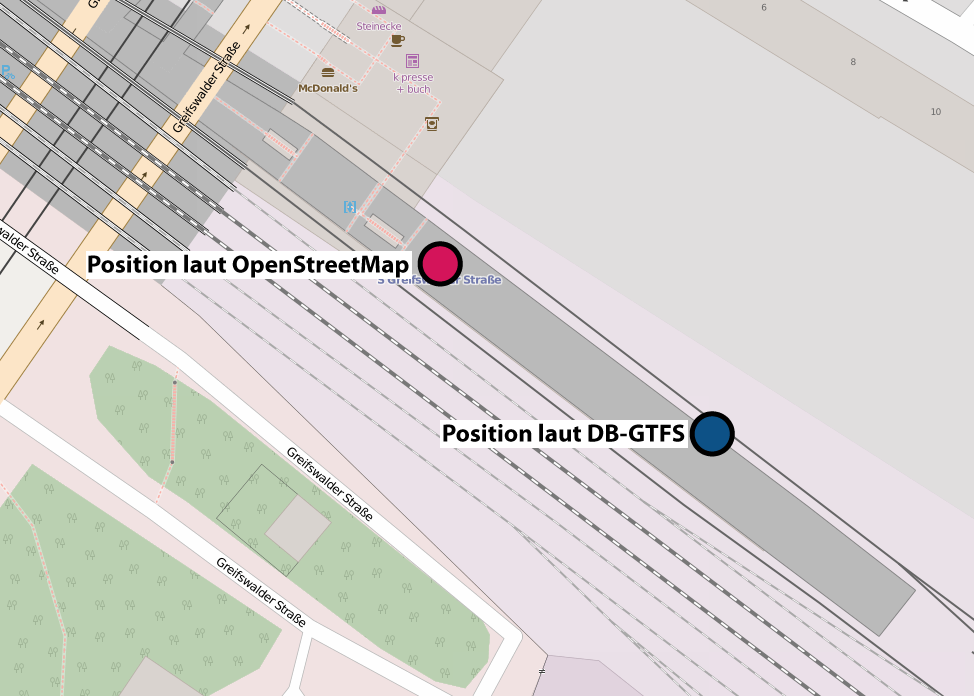
\includegraphics[width=0.7\textwidth]{gfx/gtfs2osm_geoDiff.png}}
   \caption{Abweichung der geographischen Position in beiden Datenbanken am Beispiel S-Bahnhof Greifswalder Straße Berlin}
   \label{fig:gtfs2osm:geoDiff}
 \end{figure}
Ebensowenig konnte eine Bereichssuche genutzt werden, da nicht zusammengehörige Bahnhofsobjekte teilweise sehr nah beieinander, zusammengehörige Bahnhofsobjekte jedoch auch sehr fern voneinander weg liegen und hier kein exakter Grenzwert gefunden werden konnte. In Abbildung \ref{fig:gtfs2osm:nearNameDiff} sind die beiden zusammengehörigen Bahnhofsobjekte ``Berlin-Wuhlheide'' sowie ``S-Wuhlheide'' nur knapp näher beieinander als das fremde Bahnhofsobjekt ``Wuhlheide-Parkeisenbahn''. Hier müsste man die Grenze bei ca. 100m ziehen. In Abbildung \ref{fig:gtfs2osm:farLikelihood} benötigt man jedoch ca. 120m um die Zugehörigkeit zu erzeugen. Daraus folgt, dass die Entfernung allein ebenfalls kein Kriterium sein kann.
\begin{figure}[htb]
   \centering
   \fbox{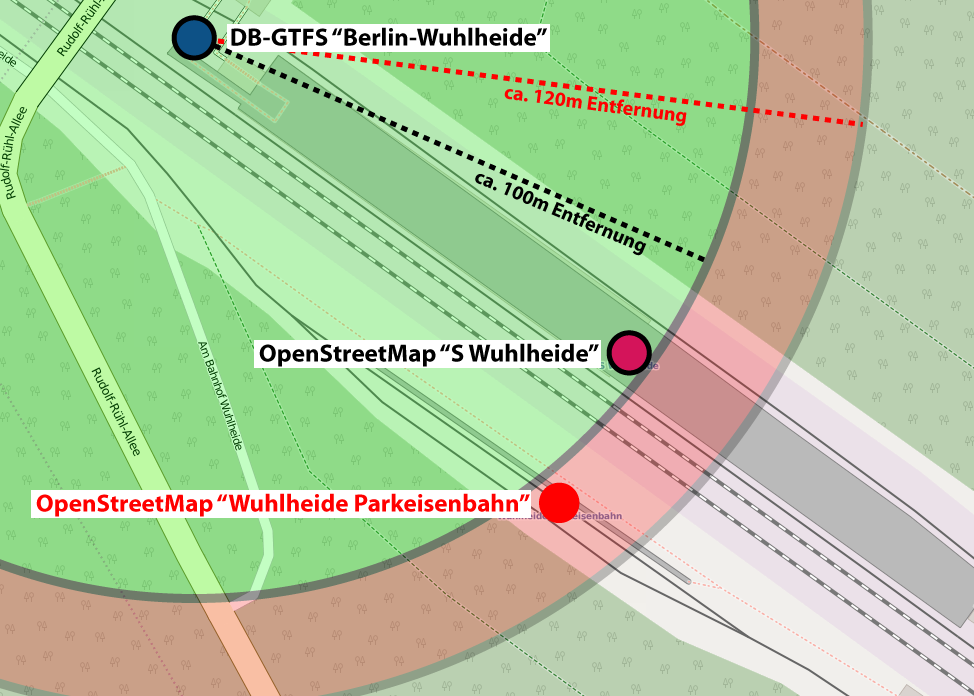
\includegraphics[width=0.7\textwidth]{gfx/gtfs2osm_nearNameDiff.png}}
   \caption{Entfernungen zwischen zusammengehörigen und nicht zusammengehörigen Bahnhofsobjekten}
   \label{fig:gtfs2osm:nearNameDiff}
 \end{figure}
 \begin{figure}[htb]
   \centering
   \fbox{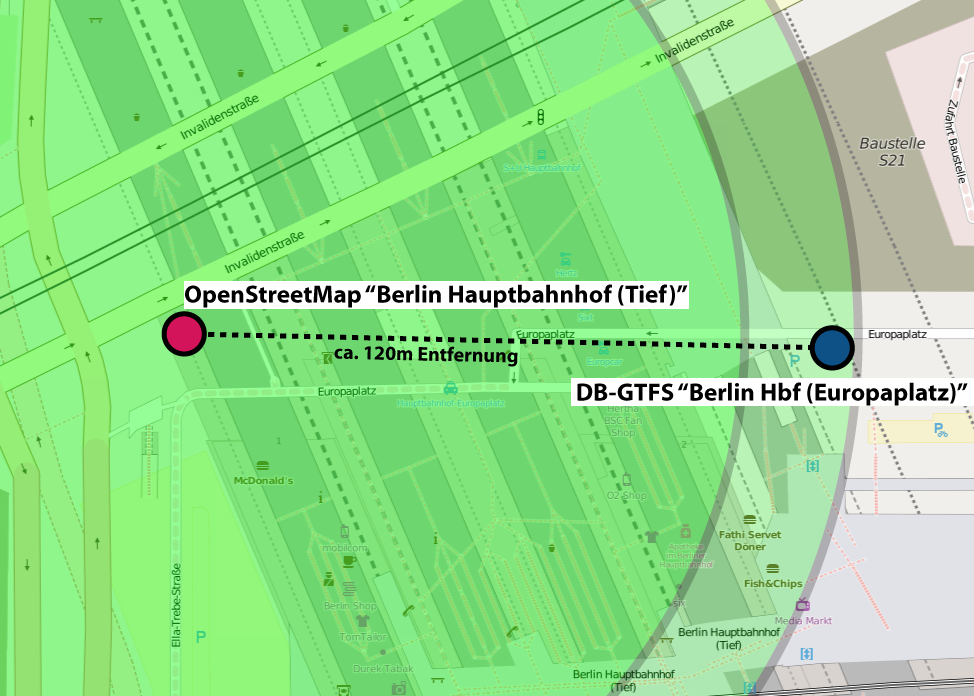
\includegraphics[width=0.7\textwidth]{gfx/gtfs2osm_farLikelihood.png}}
   \caption{Entfernungen zwischen zusammengehörigen Bahnhofsobjekten 120m}
   \label{fig:gtfs2osm:farLikelihood}
 \end{figure}

Der Name konnte ebenfalls nicht alleinstehend als Schlüssel verwendet werden. Zum Beispiel existiert in den DB-GTFS Daten ein Objekt names ``Berlin Hbf'' und in den OpenStreetMap Daten ein Objekt names ``S Hauptbahnhof''. Diese Objekte gehören zusammen, ihre Bezeichnungen sind jedoch stark unterschiedlich.

Mir wurde klar, dass ich die Klassifikation nur durch die Kombination beider Attribute (Name sowie geographische Entfernung) vornehmen konnte. Zum Vergleich der String-Ähnlichkeit entschied ich mich für eine normalisierte Variante der \textit{Levenshtein-Distanz}, welche einen Wert im Interval $[0,1]$ ermittelt.
$0$ bedeutet dass beide Strings gleich, und $1$ dass beide Strings vollständig unterschiedlich sind.
Details zur genauen Methode finden sich in Anhang \ref{sec:appendix:levenshtein}.

Da es sich um ein Klassifikationsproblem handelte, unternahm ich Versuche das Problem mit einem \textit{Naive Bayse-Klassifikator} zu lösen.
Diesen implementierte ich zusammen mit meinem Betreuuer in der Programmiersprache \texttt{R}.
Auf den Klassifikator in \texttt{R} wird an dieser Stelle nicht weiter eingegangen, da der Aufwand, diesen anschließend in das Java-Programm zu integrieren in keinem Verhältnis zum Nutzen stand.
Jedoch half mir der, speziell für den Klassifikator erstellte, Trainingsdatensatz (siehe Tabelle \ref{tab:gtfs2osm:trainingset}), gute Schwellwerte der beiden Merkmale Namensgleichheit und Entfernung zu finden.

\begin{table}[]
\small
\centering
\caption{Beispiel aus dem erstellten Trainingsdatensatz zur Klassifikation zusammenhängender Bahnhofsobjekte}
\label{tab:gtfs2osm:trainingset}
\begin{tabular}{|l|l|l|l|l|}
\hline
\textbf{gtfs}             & \textbf{osm}        & \textbf{levenshtein} & \textbf{geoDistance} & \textbf{match} \\ \hline
Bernauer Str. (U), Berlin & U Bernauer Straße   & 0,125                & 0,0008372348         & TRUE           \\ \hline
Bernauer Str. (U), Berlin & U Voltastraße       & 0,6136363636         & 0,0053660279         & FALSE          \\ \hline
Bernauer Str. (U), Berlin & U Rosenthaler Platz & 0,6242424242         & 0,0097482731         & FALSE          \\ \hline
Bernauer Str. (U), Berlin & S Nordbahnhof       & 0,7965367965         & 0,0099496517         & FALSE          \\ \hline
Yorckstr. (S+U), Berlin   & U Yorckstraße       & 0,3164983165         & 0,0002386729         & TRUE           \\ \hline
...                       & ...                 & ...                  & ...                  & ...            \\ \hline
\end{tabular}
\end{table}

Ich erstellte ein Hilfsprogramm, welches verschiedene Kombinationen aus Schwellwerten testete. Nachdem es versucht hatte eine Zusammengehörigkeit vorherzusagen, wurden die Kennzahlen \textit{Precision (Genauigkeit)}, \textit{Recall (Trefferquote)} und das \textit{F-Maß} berechnet. Dies sind Kennzahlen zur qualitativen Bewertung eines Klassifikators. (Näheres hierzu in Anhang \ref{sec:appenix:fmeasure}).

Die beste Vorhersage, ob zwei Bahnhöfe zusammengehörten, erzielte ich, wenn die Levenshtein-Distanz $\leq0,825$ und die geographische Distanz $\leq0,0045$ war. Diese Kombination erzielte auf dem Trainingsdatensatz das beste F-Maß mit einem Wert von $0,9842$.

Nun hatte ich eine Lösung, mit der ich die zu einem DB-GTFS Bahnhofsobjekt zugehörigen OpenStreetMap Bahnhofsobjekte finden konnte. Jedoch gab es innerhalb der DB-GTFS Daten auch teilweise mehrere Bahnhofsobjekte pro Bahnhof.
Dies löste ich, in dem ich einen Bahnhof als Sammlung aus verschiedenen DB-GTFS-, sowie OpenStreetMap Objekten verstand.
Diese Sammlungen repräsentierte ich als \texttt{StationCluster}-Objekte (siehe Abbildung \ref{fig:gtfs2osm:stationcluster}).

\begin{figure}[htb]
   \centering
   \fbox{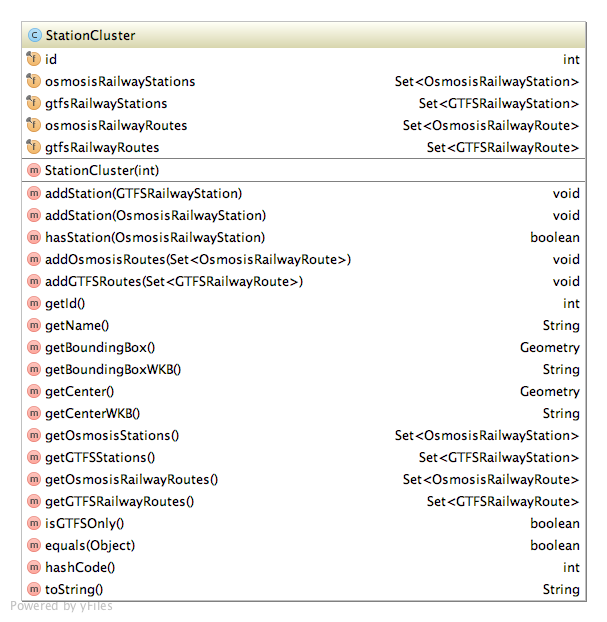
\includegraphics[width=0.7\textwidth]{gfx/gtfs2osm_stationcluster.png}}
   \caption{Die Klasse StationCluster}
   \label{fig:gtfs2osm:stationcluster}
 \end{figure}

Um diese zu befüllen, iterierte ich über alle DB-GTFS Objekte und ermittelte pro Objekt alle zugehörigen OpenStreetMap Objekte.
Anschließend prüfte ich, ob bereits ein \texttt{StationCluster} existiert, der eins dieser OpenStreetMap Objekte enthält.
Wenn ja, dann wurden die DB-GTFS-, sowie die OpenStreetMap Objekte diesem \texttt{StationCluster} hinzugefügt.
Wenn nicht, dann wurde ein neuer \texttt{StationCluster} angelegt.

Die so erzeugten \texttt{StationCluster} Objekte waren nun das Kernstück meines Ergebnisses und wurden in die Ausgabedatei exportiert. Des Weiteren wurde pro Gruppe ein neuer Name erzeugt und Koordinaten ermittelt, welche den Mittelpunkt aller Objekte sowie das umschließende Rechteck abbilden.

Ein Ergebnisbeispiel findet sich in Anhang \ref{sec:appendix:gtfs2osm_example}.

\subsubsection{Programmstruktur}

Es wurden erneut externe Bibliotheken (siehe Tabelle \ref{tab:GTFS2OSM:Libraries}) verwendet.
\begin{table}[htb]
\small
\centering
\caption{verwendete externe Bibliotheken}
\label{tab:GTFS2OSM:Libraries}
\begin{tabular}{|l|l|}
\hline
\textbf{Problem}                          & \textbf{verwendete Bibliothek}     \\ \hline
Datenbankanbindung PostgreSQL             & PostgreSQL JDBC Driver JDBC 4.1    \\ \hline
Verarbeitung von Kommandozeilenargumenten & Apache Commons CLI                 \\ \hline
Ermittlung von String-Distanzen           & info.debatty.java-string-similarity         \\ \hline
Ermittlung von Geo-Distanzen           & Vivid Solutions Inc. JTS Topology Suite         \\ \hline
erweiterte Datenstrukturen, z.B. Tabellen & Google Guava          \\ \hline
\end{tabular}
\end{table}

Das Programm erhielt den Namen \texttt{GTFS2OSMRailwayLinker}.
Die Struktur des kompletten Programms ist in Abbildung \ref{fig:gtfs2osm:uml_full} ersichtlich.
Die Klasse \texttt{Main} erzeugt einen \texttt{CSVExporter}, welcher für den Export ins CSV-Format verantwortlich ist.
Anschließend werden die Datenbankschnittstellen \texttt{GTFSDB} und \texttt{OsmosisDB}, sowie der, für die Gruppenbildung zuständige, \texttt{Clusterizer} angelegt.
Dies ist in Abbildung \ref{fig:gtfs2osm:uml_main} zu erkennen.
Der \texttt{Clusterizer} iteriert nun über die DB-GTFS Objekte und legt \texttt{StationCluster} an (siehe Abbildung \ref{fig:gtfs2osm:uml_stationcluster}).
Diese werden letztendlich über den \texttt{CSVExporter} exportiert.

\begin{figure}[H]
   \centering
   \fbox{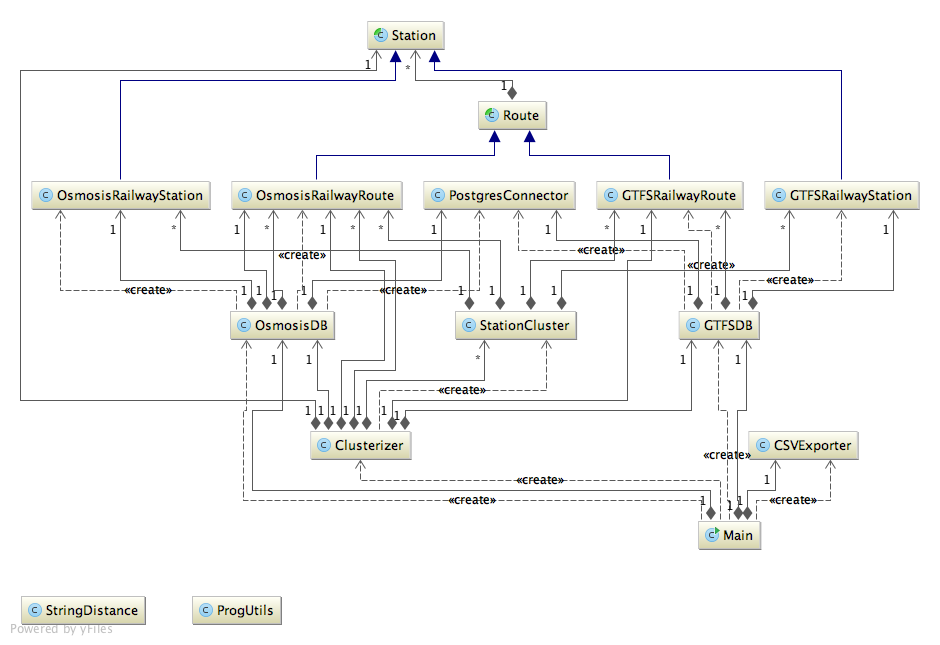
\includegraphics[width=1\textwidth]{gfx/gtfs2osm_uml_full.png}}
   \caption{Klassendiagramm GTFS2OSMRailwayLinker}
   \label{fig:gtfs2osm:uml_full}
 \end{figure}

\begin{figure}[H]
   \centering
   \fbox{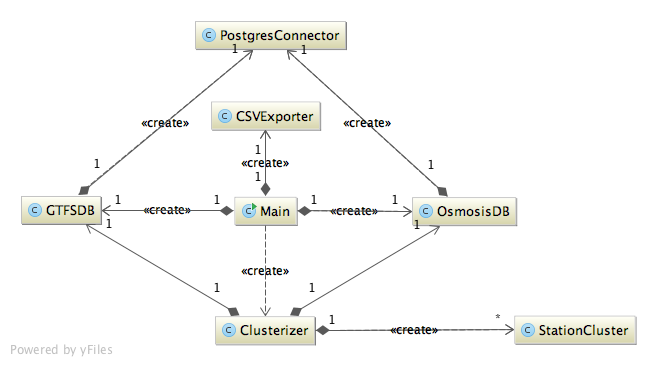
\includegraphics[width=1\textwidth]{gfx/gtfs2osm_uml_main.png}}
   \caption{Auszug aus dem Klassendiagramm GTFS2OSMRailwayLinker Fokus auf Main}
   \label{fig:gtfs2osm:uml_main}
 \end{figure}


\begin{figure}[H]
   \centering
   \fbox{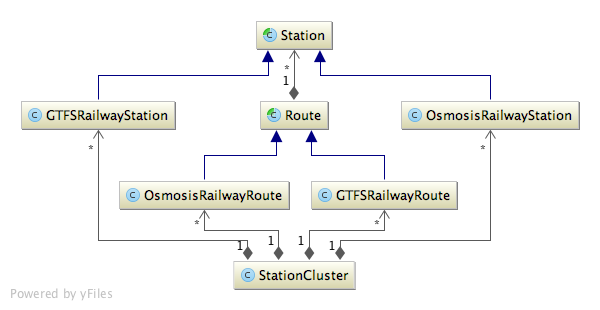
\includegraphics[width=1\textwidth]{gfx/gtfs2osm_uml_stationcluster.png}}
   \caption{Auszug aus dem Klassendiagramm GTFS2OSMRailwayLinker Fokus auf StationCluster}
   \label{fig:gtfs2osm:uml_stationcluster}
 \end{figure}

\subsubsection{Schwierigkeiten}

Als Nebenaufgabe sollte geprüft werden, inwiefern sich aus den kombinierten Daten ein geographisch exakter Streckenverlauf eines Zuges für die graphische Darstellung ermitteln lässt.
Nach zahlreichen Versuchen stellte sich heraus, dass dies mit den gegebenen Daten nicht möglich ist.
Die Versuche nahmen sehr viel Zeit in Anspruch.
Zwar sind aus den DB-GTFS Daten die einzelnen Bahnhöfe pro Linie ableitbar, jedoch existiert keine zuverlässige Information über den exakten Streckenverlauf.
Das Hauptproblem an dieser Stelle ist, dass das Streckennetz der Deutschen Bahn nur eine Art Straßenkarte ist.
Es existieren keine öffentlich zugänglichen Informationen, aus denen der genaue Verlauf, zum Beispiel eines bestimmten Fernzuges, ersichtlich ist.

\subsection{Datenaufwertung und Datenaufbereitung}
Zum Ende meiner Praxisphase bekam ich noch mehrere kleine Aufgaben.
Hauptsächlich ging es hier um Aufwertung von Daten oder dem gezielten Export von Daten aus offenen Datenquellen.

Beispielsweise wurde die Aufgabe gestellt, alle Angaben zur Bevölkerungsgröße aus \textit{Wikidata}\footnote{www.wikidata.org} zu extrahieren.
Hierzu lud ich mir eine Kopie der aktuellen Wikidata-Datenbank herunter.
Diese im JSON-Format vorliegende Datei wurde anschließend mit einem Python-Script nach den gesuchten Daten durchsucht und die Ergebnisse in eine CSV-Datei exportiert.

Eine weitere Aufgabe war es, eine Datenquelle für alle politischen Grenzen der Welt zu suchen und gegebenenfalls eine Datei, welche diese beinhaltet, zu erstellen.
Nach einer Recherche stellte ich fest, dass solche Daten zwar kostenfrei für Staatsgrenzen zur Verfügung stehen (zum Beispiel von \textit{GeoNames}\footnote{http://www.geonames.org}), jedoch sind Daten für kleinere administrative Bereiche wie zum Beispiel Bundesländer nicht kostenfrei auffindbar.
Meine Idee war es nun, dies mit OpenStreetMap Daten zu lösen. In Abschnitt~\ref{osm2pgsql} auf Seite~\pageref{osm2pgsql} erwähnte ich bereits das Werkzeug \textbf{osm2pgsql}\footnote{https://github.com/openstreetmap/osm2pgsql}.
Eine, mit diesem Werkzeug importierte, OpenStreetMap Datenbank eignet sich sehr gut zur Extraktion administrativer und politischer Grenzen, da der Hauptzweck der importierten Datenbank das Rendern von Karten ist.
Hier wurde innerhalb von osm2pgsql viel Wert auf saubere Erzeugung von Grenzen gelegt.
Da ein Import der kompletten \textit{planet.osm} Datei jedoch zu viel Platz in Anspruch nahm, wurde die Grenzextraktion nur exemplarisch anhand der, bereits beim DFKI vorliegenden, deutschen Datenbasis durchgeführt.
